\section{Local Linear/Polynomial Regression}

  Now another way to think about the kernel estimator is as such. Suppose that you're doing linear regression on a bunch of points and you want to choose a $c$ that minimizes the loss. 
  \begin{equation}
    \sum_i (Y_i - c)^2
  \end{equation}

  You would just pick $c = \hat{Y}$. But if you are given some sort of locality condition, that the value of $c$ should depend more on the values closer to it, you're really now minimizing 
  \begin{equation}
    \sum_i (Y_i - c(x))^2 K \bigg( \frac{X_i - x}{h} \bigg)
  \end{equation}

  Minimizing this by setting the derivative equal to $0$ and solving gives us the kernel estimator. Therefore you're fitting some sort of local constant at a point $X$. But why fit a local constant, when you can fit a local line or polynomial? This is the idea behind local polynomial regression.

  \begin{figure}[H]
    \centering 
    \begin{tikzpicture}[scale=1.5]
      % Axes
      \draw[thick] (-2.5,0) -- (2.5,0);
      \draw[thick] (0,-0.5) -- (0,2);

      % X label
      \node[below] at (0.9,-0.3) {$x$};
      \draw[thick, gray, dashed] (0.9,-0.1) -- (0.9,2.1);

      % Gaussian-shaped dotted curve
      \draw[dotted, thick, domain=-2:2, samples=100] plot (\x, {1.2*exp(-0.8*\x*\x) + 0.5});

      % Red linear line
      \draw[red, thick] (0,1.88) -- (1.6,0.53);

      % Blue horizontal line labeled c
      \draw[blue, thick] (0.5,1.1) -- (1.3,1.1);

      % Gaussian curve at bottom
      \draw[thick, domain=0:1.8, samples=100] plot (\x, {0.3*exp(-5*(\x - 0.9)*(\x-0.9))});
    \end{tikzpicture}
    \caption{Rather than using a local constant (blue), we can use a local linear estimator (red).} 
    \label{fig:local_linear_estimator}
  \end{figure}

  Therefore, we can minimize the modified loss. 

  \begin{definition}[Local Polynomial Estimator]
    The \textbf{local polynomial estimator} is a local linear kernel smoother that estimates the function $\hat{f}$ that minimizes the following loss. 
    \begin{equation}
      \argmin_{\beta} \sum_i K \bigg( \frac{X_i - x}{h} \bigg) \big( Y_i - \beta_0 (x) - \beta_1 (x) (x- X_i)\big)
    \end{equation}
  \end{definition}

  So we can fit a line 
  \begin{equation}
    f(\mu) \approx \hat{\beta}_0 (x) + \hat{\beta}_1 (x) (\mu - x)
  \end{equation}
  and simply remove the intercept term to get the local linear estimator. 
  \begin{equation}
    \hat{f}(x) = \hat{\beta}_0 (x)
  \end{equation}
  Note that this is not the same as taking the constant estimate. We are extracting the fitted intercept term and so $\hat{\beta}_0(x) \neq c(x)$. 

\subsection{Weighted Least Squares Solution}

  It turns out that this has an analytic solution. Looking the local polynomial loss should tell you that we're really doing OLS, but weighting the points differently. This sounds a lot like weighted least squares. 

  \begin{theorem}[Weighted Least Squares]
    The solution to the local linear estimator is similar to the weighted least squares solution. 
    \begin{equation}
      \hat{\beta}(x) = \begin{pmatrix} \hat{\beta}_0 (x) \\ \hat{\beta}_1 (x) \end{pmatrix} = (X_x^T W_x X_x)^{-1} X_x^T W_x Y
    \end{equation}
    where we have put the subscript $x$ to emphasize that the matrices are dependent on $x$, and 
    \begin{equation}
      X_x = \begin{pmatrix} 1 & X_1 - x \\ \vdots & \vdots \\ 1 & X_n - x \end{pmatrix} \qquad W_x = \begin{pmatrix} K \big( \frac{X_1 - x}{h} \big) & 0 & \cdots & 0 \\ 0 & K \big( \frac{X_2 - x}{h} \big) & \cdots & 0 \\ \vdots & \vdots & \ddots & \vdots \\ 0 & 0 & \cdots & K \big( \frac{X_n - x}{h} \big) \end{pmatrix}
    \end{equation}
  \end{theorem}

  Remember that at the end, once you compute $\hat{\beta}$, take the intercept term and your estimate is actually $\hat{\beta}_0$. Note that this of the form $(X_x^T W_x X_x)^{-1} X_x^T W_x Y = LY$, and so this is a linear smoother. 

\subsection{Bias Variance Decomposition}

  Computationally, it's similar to kernel regression and it gets rid of both the boundary and design bias. Let's see this mathematically. 

  \begin{theorem}[Bias Variance Decomposition]
    Under some regularity conditions, the risk of $\hat{m}$ is
    \begin{equation}
      \frac{h^4}{4} \int \left( \text{tr}(m^{\prime\prime}(x) \int K(u)uu^T du) \right)^2 dP(x) + \frac{1}{nh_d} \int K^2(u)du \int \sigma^2(x)dP(x) + o(h_n^4 + (nh_n^d)^{-1})
    \end{equation}
  \end{theorem}
  \begin{proof}
    For a proof, see Fan \& Gijbels (1996). 
  \end{proof}

  For points near the boundary, the bias is $Ch^2m^{\prime\prime}(x) + o(h^2)$ whereas, the bias is $Chm^{\prime}(x) + o(h)$ for kernel estimators.

  \begin{figure}[H]
    \centering 
    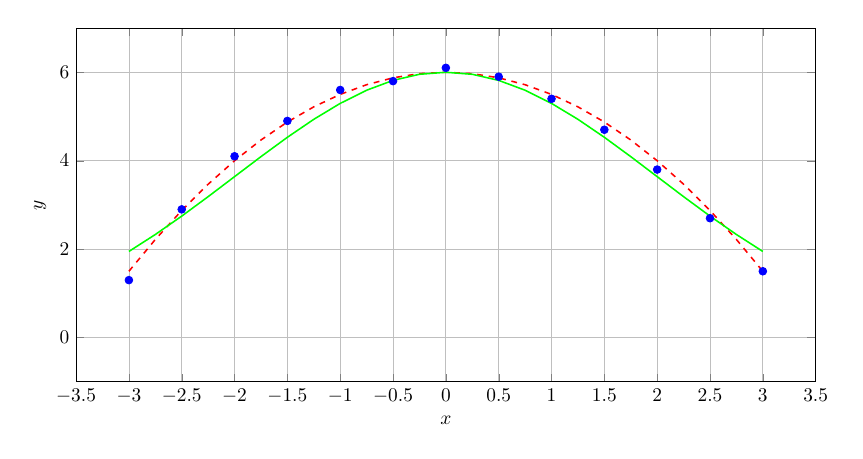
\begin{tikzpicture}[scale=0.7]
      \begin{axis}[ xlabel={$x$}, ylabel={$y$}, grid=major, width=15cm, height=8cm, domain=-3:3, xmin=-3.5, xmax=3.5, ymin=-1, ymax=7 ]

      % Plot scattered points that roughly follow the quadratic pattern
      \addplot[only marks, mark=*, mark size=2pt, blue] coordinates {
        (-3, 1.3)
        (-2.5, 2.9)
        (-2, 4.1)
        (-1.5, 4.9)
        (-1, 5.6)
        (-0.5, 5.8)
        (0, 6.1)
        (0.5, 5.9)
        (1, 5.4)
        (1.5, 4.7)
        (2, 3.8)
        (2.5, 2.7)
        (3, 1.5)
      };
     
      % The quadratic curve
      \addplot[red, thick, dashed] {6 - 0.5*x^2};
     
      % Gaussian-looking curve
      \addplot[green, thick] {6*exp(-x^2/8)};
     
      \end{axis}
    \end{tikzpicture}
    \caption{Diagram of the boundary bias. The green line represents what you would see for a fitted kernel regressor. At the boundaries (endpoints of the data), you can see that because the kernel is cut off, more and more bias accumulates. We avoid this in local polynomial regression.} 
  \end{figure}

\subsection{Local Polynomial Regression}

  We can extend this and compute local polynomials rather than lines. 

  \begin{definition}[Local Polynomial Estimator]
    The \textbf{local polynomial estimator} is a local linear kernel smoother that estimates the function $\hat{f}$ that minimizes the following loss. 
    \begin{equation}
      \argmin_{\beta} \sum_i K \bigg( \frac{X_i - x}{h} \bigg) \big( Y_i - (\beta_0 (x) - \beta_1 (x) (x- X_i) + \ldots + \beta_k (x) (x - X_i)^k )\big)
    \end{equation}
  \end{definition}

  People do this because there is also bias in the peaks and troughs of the data, and local quadratics can capture this much better. Beyond quadratics, there's not much more benefits and we have the accumulating cost of variance. 
